\documentclass[xcolor={table}]{beamer}
\usepackage{fleqn}
\usepackage{graphicx}
\usepackage{coordsys} %for \numbline commander

%Setup appearance:
\usetheme{Darmstadt}
\usefonttheme[onlylarge]{structurebold}
\setbeamerfont*{frametitle}{size=\normalsize,series=\bfseries}
\setbeamertemplate{navigation symbols}{}
\setbeamertemplate{bibliography item}{[\theenumiv]}

% Standard packages
\usepackage[english]{babel}
\usepackage[latin1]{inputenc}
\usepackage{times}
\usepackage[T1]{fontenc}
\usepackage{multirow}
\usepackage{subfigure}
\usepackage{pbox}
\usepackage{arydshln}
\usepackage{pifont}
\usepackage{cancel}
\usepackage{rotating} % for sideways headings

% Source Code packages
\usepackage{algorithm2e}
\usepackage{algorithmic}

\DeclareSymbolFont{extraup}{U}{zavm}{m}{n}
\DeclareMathSymbol{\varclub}{\mathalpha}{extraup}{84}
\DeclareMathSymbol{\varspade}{\mathalpha}{extraup}{85}
\DeclareMathSymbol{\varheart}{\mathalpha}{extraup}{86}
\DeclareMathSymbol{\vardiamond}{\mathalpha}{extraup}{87}

%%% This section command that adds a big page with section dividers
\usepackage{xifthen}% provides \isempty test
\newcommand{\SectionSlide}[2][]{
	\ifthenelse{\isempty{#1}}
		{\section{#2}\begin{frame} \begin{center}\begin{huge}#2\end{huge}\end{center}\end{frame}}
		{\section[#1]{#2}\begin{frame} \begin{center}\begin{huge}#2\end{huge}\end{center}\end{frame}}
}
%Extends the section slide to to include a shortened section title for the navigation bar as a second parameter
\newcommand{\SectionSlideShortHeader}[3][]{
	\ifthenelse{\isempty{#1}}
		{\section[#3]{#2}\begin{frame} \begin{center}\begin{huge}#2\end{huge}\end{center}\end{frame}}
		{\section[#1]{#2}\begin{frame} \begin{center}\begin{huge}#3\end{huge}\end{center}\end{frame}}
}

\newcommand{\refer}[1]{\footnote{#1}}
\newcommand{\GW}{\text{\textit{Guess-Who~}}}
\newcommand{\keyword}[1]{\alert{\textbf{#1}}\index{#1}}
\newcommand{\firstkeyword}[1]{\textbf{#1}\index{#1}}
\newcommand{\indexkeyword}[1]{\alert{\textbf{#1}\index{#1}}}
\newcommand{\featN}[1]{\textsc{#1}}
\newcommand{\featL}[1]{\textit{'#1'}}
 \newcommand{\ourRef}[1]{\ref{#1} $^{\text{\tiny[\pageref{#1}]}}$}
 \newcommand{\ourEqRef}[1]{\eqref{#1}$^{\text{\tiny[\pageref{#1}]}}$}
  
\DeclareMathOperator*{\argmax}{argmax}
\DeclareMathOperator*{\argmin}{argmin}

\title{Appendix A Descriptive Statistics and Data Visualization for Machine learning}
	\author{John D. Kelleher and Brian Mac Namee and Aoife D'Arcy}
	\institute{}
	\date{}

\begin{document}
\begin{frame}
	\titlepage
\end{frame}
\begin{frame}
	 \tableofcontents
\end{frame}


\SectionSlideShortHeader{Descriptive Statistics}{Descriptive Statistics}

\subsection{Descriptive Statistics for Continuous Features}

\begin{frame} 
\begin{itemize}
\item The \keyword{arithmetic mean} (or \keyword{sample mean} or just \keyword{mean}) of a set of $n$ values for a feature $a$, $a_1, a_2 \ldots a_n$, is denoted by the symbol $\overline{a}$, and is calculated as: 
\end{itemize}

\begin{center}
\begin{equation*}\centering
\overline{a}=\frac{1}{n} \displaystyle \sum_{i=1}^{n} a_i
\label{eq:sample_mean}
\end{equation*}
\end{center}

\end{frame} 

\begin{frame} 
	\begin{example}
 		\begin{table}[!htb]
			\label{table:BasketballTeamHeights}
			\centering
			\begin{footnotesize}
			\begin{tabular}{ r | c c c c c c c c}
			\textbf{ID} & 1 & 2 & 3 & 4  & 5 & 6 & 7 & 8 \\
			\hline
			\textbf{Height} & 150 & 163 & 145 & 140 & 157 & 151 & 140 & 149 \\
			\end{tabular}
			\end{footnotesize}
		\end{table}
		\begin{figure}
			\centering
			\includegraphics[width=0.45\textwidth]{./images/DataEx-DesriptiveStatsPuppetShowAveragePlusHeights.pdf}
			\caption{The members of a school basketball squad. The dashed grey line shows the arithmetic mean of the players' heights.}
			\label{fig:descriptiveStatsTeam}
		\end{figure}
	\end{example}
\end{frame} 

\begin{frame} 
	\begin{example}
 		\begin{table}[!htb]
			\label{table:BasketballTeamHeights}
			\centering
			\begin{footnotesize}
			\begin{tabular}{ r | c c c c c c c c}
			\textbf{ID} & 1 & 2 & 3 & 4  & 5 & 6 & 7 & 8 \\
			\hline
			\textbf{Height} & 150 & 163 & 145 & 140 & 157 & 151 & 140 & 149 \\
			\end{tabular}
			\end{footnotesize}
		\end{table}
		\begin{figure}
			\centering
			\includegraphics[width=0.45\textwidth]{./images/DataEx-DesriptiveStatsPuppetShowAveragePlusHeights.pdf}
			\caption{The members of a school basketball squad. The dashed grey line shows the arithmetic mean of the players' heights.}
			\label{fig:descriptiveStatsTeam}
		\end{figure}
		\begin{small}
			\begin{alignat*}{2}
				\overline{\featN{Height}} & =  \frac{1}{8}\times\left(150 + 163 + 145 + 140 + 157 + 151 + 140 + 149\right) \\
				 & =   149.375
			\end{alignat*}
		\end{small}
	\end{example}
\end{frame} 


\begin{frame} 
	\begin{itemize}
		\item The \indexkeyword{arithmetic mean} is one measure of the \indexkeyword{central tendency} of a \keyword{sample} (for our purposes a sample is just a set of values for a feature in an ABT). 
		\item Any measure of \indexkeyword{central tendency} is, however, just an approximation. 
	\end{itemize}
\end{frame} 

\begin{frame} 
	\begin{example}
		\begin{itemize}
			\item Suppose our basketball squad manage to sign a \textit{ringer} measuring in at $229$cm 
		\end{itemize}
		\begin{figure}[!htb]
			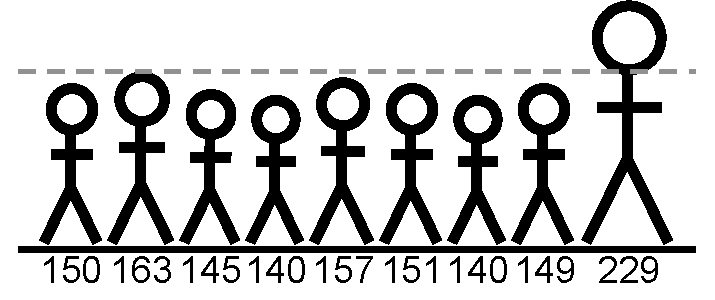
\includegraphics[width=0.45\textwidth]{./images/DataEx-DesriptiveStatsPuppetShowBigManPlusHeightsFixed}
			\label{fig:descriptiveStatsTeamExtraBigMan}
		\end{figure}
		\begin{itemize}
			\item The arithmetic mean for the full group is $158.235$cm and no longer represents the central tendency of the group.  
			\item An unusually large or small value like this is referred to as an \keyword{outlier} - the arithmetic mean is very sensitive to outliers. 
		\end{itemize}
	\end{example}
\end{frame} 

\begin{frame} 
\begin{itemize}
\item The \keyword{median} of a set of values can be calculated by ordering the values from lowest to highest and selecting the middle value. 
\item If there is an even number of values in the sample then the median is obtained by calculating the arithmetic mean of the middle two values. 
\end{itemize}
\end{frame} 

\begin{frame}
	\begin{example}
		\begin{figure}[!htb]
			\includegraphics[width=0.45\textwidth]{./images/DataEx-DesriptiveStatsPuppetShowMedianPlusHeights.pdf}
			\caption{The members of the school basketball squad ordered by height, the dashed grey line shows the \indexkeyword{median}.}
			\label{fig:descriptiveStatsTeamExtraMedian}
		\end{figure}
		\begin{table}[!htb]
			\label{table:BasketballTeamHeightsExtraOrdered}
			\centering
			\begin{footnotesize}
			\begin{tabular}{ r | c c c c c c c c c}
			\textbf{ID} & 4 & 7 & 3 & 8  & 1 & 6 & 5 & 2 & 9\\
			\hline
			\textbf{Height} & $140$ & $140$ & $145$ & $149$ & $\mathbf{\underline{150}}$ & $151$ & $157$ & $163$ & $229$ \\
			\end{tabular}
			\end{footnotesize}
		\end{table}
	\end{example}
\end{frame} 



\begin{frame} 
\begin{itemize}
\item We also measure the \keyword{variation} in our data. 
\item In essence, most of statistics, and in turn analytics, is about describing and understanding variation. 
\end{itemize}
\end{frame} 


 \begin{frame} 
 \begin{itemize}
 \item The simplest measure of variation is the \keyword{range}:
 \end{itemize}
 
\begin{equation*}
\centering
\text{range}=max(a) - min(a)
\label{eq:range}
\end{equation*}
\end{frame} 

 \begin{frame} 
	\begin{example}
	What is the range of the heights of the two basketball squads?
 		\begin{table}[!htb]
			\label{table:BasketballTeamHeights}
			\centering
			\begin{footnotesize}
			\begin{tabular}{ r | c c c c c c c c}
			\textbf{ID} & 1 & 2 & 3 & 4  & 5 & 6 & 7 & 8 \\
			\hline
			\textbf{Height} & 150 & 163 & 145 & 140 & 157 & 151 & 140 & 149 \\
			\end{tabular}
			\end{footnotesize}
		\end{table}
		\begin{table}
		\label{table:BasketballTeamHeights2}
		\centering
		\begin{footnotesize}
		\begin{tabular}{ r |  c c c c c c c c }
		\textbf{ID} & 1 & 2 & 3 & 4  & 5 & 6 & 7 & 8 \\
		\hline
		\textbf{Height} & $192$ & $102$ & $145$ & $165$ & $126$ & $154$ & $123$ & $188$ \\
		\end{tabular}
		\end{footnotesize}
		\end{table}
\end{example}
\end{frame} 

 \begin{frame} 
	\begin{example}
	What is the range of the heights of the two basketball squads?
	\begin{equation*}
	\centering
	\text{range}=163 - 140 = 23
	\label{eq:range}
	\end{equation*}
	\begin{equation*}
	\centering
	\text{range}=192 - 102 = 90
	\label{eq:range}
	\end{equation*}
\end{example}
\end{frame} 




\begin{frame} 
\begin{itemize}
\item The \keyword{variance} of a sample measures the average difference between each value in a sample and the mean of that sample. 
\item The \indexkeyword{variance} of the $n$ values of a feature $a$, $a_1, a_2 \ldots a_n$, is denoted $var(a)$ and is calculated as: 
\end{itemize}
\begin{equation*}
var(a)= \displaystyle\frac{\displaystyle\sum_{i=1}^{n} \left( a_i - \overline{a} \right)^2}{n-1}
\label{eq:sample_variance}
\end{equation*}
\end{frame} 



 \begin{frame} 
\begin{example}
What is the variance of the heights of the two basketball squads?
 		\begin{table}[!htb]
			\label{table:BasketballTeamHeights}
			\centering
			\begin{footnotesize}
			\begin{tabular}{ r | c c c c c c c c}
			\textbf{ID} & 1 & 2 & 3 & 4  & 5 & 6 & 7 & 8 \\
			\hline
			\textbf{Height} & 150 & 163 & 145 & 140 & 157 & 151 & 140 & 149 \\
			\end{tabular}
			\end{footnotesize}
		\end{table}
		\begin{table}
		\label{table:BasketballTeamHeights2}
		\centering
		\begin{footnotesize}
		\begin{tabular}{ r |  c c c c c c c c }
		\textbf{ID} & 1 & 2 & 3 & 4  & 5 & 6 & 7 & 8 \\
		\hline
		\textbf{Height} & $192$ & $102$ & $145$ & $165$ & $126$ & $154$ & $123$ & $188$ \\
		\end{tabular}
		\end{footnotesize}
		\end{table}
\end{example}
\end{frame} 

\begin{frame} 
\begin{example}
\begin{scriptsize}
\begin{alignat*}{2}
var(\featN{Height}) & =  \frac{\left( 150 - 149.375 \right)^2 + \left(163 - 149.375 \right)^2 + \ldots + \left(149 - 149.375 \right)^2}{8-1} \\ 
 & =  63.125
\end{alignat*}


\begin{alignat*}{2}
var(\featN{Height}) & =  \frac{\left(192 - 149.375 \right)^2 + \left(102 - 149.375 \right)^2 + \ldots + \left(188 - 149.375 \right)^2}{8-1} \\
  & =  1,011.41071
\end{alignat*}
\end{scriptsize}

\end{example}

\end{frame} 



 \begin{frame} 
 
\begin{itemize}
\item  The \keyword{standard deviation}, $sd$, of a sample is calculated by taking the square root of the \indexkeyword{variance} of the sample:
\end{itemize}
 
\begin{alignat}{2}
sd(a) & = \sqrt{var(a)} \\
 & = \sqrt{\frac{\displaystyle\sum_{i=1}^{n} \left( a_i - \overline{a} \right)^2}{n-1}}
\label{eq:sample_standard_deviation}
\end{alignat}
\end{frame} 

\begin{frame} 
\begin{example}
What is the standard deviation of the heights of the two basketball squads?
 		\begin{table}[!htb]
			\label{table:BasketballTeamHeights}
			\centering
			\begin{footnotesize}
			\begin{tabular}{ r | c c c c c c c c}
			\textbf{ID} & 1 & 2 & 3 & 4  & 5 & 6 & 7 & 8 \\
			\hline
			\textbf{Height} & 150 & 163 & 145 & 140 & 157 & 151 & 140 & 149 \\
			\end{tabular}
			\end{footnotesize}
		\end{table}
		\begin{table}
		\label{table:BasketballTeamHeights2}
		\centering
		\begin{footnotesize}
		\begin{tabular}{ r |  c c c c c c c c }
		\textbf{ID} & 1 & 2 & 3 & 4  & 5 & 6 & 7 & 8 \\
		\hline
		\textbf{Height} & $192$ & $102$ & $145$ & $165$ & $126$ & $154$ & $123$ & $188$ \\
		\end{tabular}
		\end{footnotesize}
		\end{table}
\end{example}
\end{frame} 

\begin{frame} 
\begin{example}
\begin{footnotesize}
\begin{alignat*}{2}
sd(\featN{Height}) & =  \sqrt{63.125} \\ 
 & =  7.9451\dots
\end{alignat*}
\begin{alignat*}{2}
sd(\featN{Height}) & =  \sqrt{1,011.41071} \\
  & =  31.8026\dots
\end{alignat*}
\end{footnotesize}
\end{example}
\end{frame} 

 \begin{frame} 
	\begin{itemize} 
		\item \keyword{Percentiles} are another useful measure of the variation of the values for a feature: a proportion of $\frac{i}{100}$ of the values in a sample take values equal to or lower than the $i^{th}$ percentile of that sample. 
	\end{itemize} 		
\end{frame} 

 \begin{frame} 
	\begin{itemize} 
		\item To calculate the $i^{th}$ percentile of the $n$ values of a feature $a$, $a_1, a_2 \ldots a_n$:
		\begin{itemize} 
			\item First order the values in ascending order and then multiply $n$ by $\frac{i}{100}$ to determine the $index$. 
			\item If the $index$ is a whole number we take the value at that position in the ordered list of values as the $i^{th}$ percentile. 
			\item If $index$ is not a whole number then we \indexkeyword{interpolate} the value for the $i^{th}$ percentile as: 
	\begin{small} 
	\begin{equation*}
		\centering
		i^{th} \text{percentile} = (1 - index\_f) \times a_{index\_w} + index\_f \times a_{index\_w + 1}
		\label{eq:percentiles}
	\end{equation*}
	\end{small}
			where $index\_w$ is the whole part of $index$, $index\_f$ is the fractional part of $index$ and  $a_{index\_w}$ is the value in the ordered list at position $index\_w$. 
		\end{itemize} 
	\end{itemize} 
\end{frame} 


 \begin{frame} 
 \begin{example} 
 \begin{table}
\label{table:BasketballTeamHeights2Ordered}
\centering
\begin{footnotesize}
\begin{tabular}{ r |  c c c c c c c c }
\textbf{ID} & 2 & 7 & 5 & 3  & 6 & 4 & 8 & 1 \\
\hline
\textbf{Height} & $102$ & $123$ & $126$ & $145$ & $154$ & $165$ & $188$ & $192$ \\
\end{tabular}
\end{footnotesize}
\end{table}
 \begin{figure}
\centering
\includegraphics[width=0.45\textwidth]{./images/DataEx-DesriptiveStatsPuppetShowTeam2OrderedPlusHeights.pdf}
\label{fig:descriptiveStatsTeam2Ordered}
\end{figure}
\begin{itemize}
\item What is the $25^{th}$ percentile of the heights of the basketball squad?
\item What is the $80^{th}$ percentile of the heights of the basketball squad?
\end{itemize}
\end{example}
\end{frame} 


 \begin{frame}  
 \begin{example}
\begin{itemize}
\item To calculate the $25^{th}$ percentile we first calculate $index$ as $\frac{25}{100}\times8 = 2$. So, the $25^{th}$ percentile is the second value in the ordered list which is $123$. 
\item To calculate the $80^{th}$ percentile we first calculate $index$ as $\frac{80}{100}\times8 = 6.4$. Because $index$ is not a whole number we set $index\_w$ to the whole part of $index$, $6$, and $index\_f$ to the fractional part, $0.4$. Then we can calculate the $80^{th}$ percentile as:
\end{itemize}
\begin{equation*}\centering
(1 - 0.4) \times 165 + 0.4 \times 188 = 174.2
\end{equation*}
\end{example}
\end{frame} 

\begin{frame}
\begin{itemize}
	\item We can use percentiles to describe another measure of variation know as the \keyword{inter-quartile range}. 
	\item The inter-quartile range is calculated as the difference between the $25^{th}$ percentile and the $75^{th}$ percentile.\footnote{These percentiles are also known the 	\keyword{lower quartile} (or $1^{st}$ quartile) and \keyword{upper quartile} (or $3^{rd}$ quartile) hence the name inter-quartile range. }
\end{itemize}
\end{frame}


\begin{frame}
\begin{example}
\centering
For the heights of the first basketball team the inter-quartile range is $151 - 140 = 11$, while for the second team it is $165 - 123 = 42$.
\end{example}
\end{frame}

\subsection{Descriptive Statistics for Categorical Features}

\begin{frame} 
\begin{itemize}
\item For categorical features we are interested primarily in \keyword{frequency counts} and \keyword{proportions}. 
	\begin{itemize}
		\item The frequency count of each level of a categorical feature is calculated by counting the number of times that level appears in the sample. 
		\item The proportion for each level is calculated by dividing the frequency count for that level by the total sample size. 
		\item Frequencies and proportions are typically presented in a \keyword{frequency table}.
	\end{itemize}
\item The \keyword{mode} is a measure of the central tendency of a categorical feature and is simply the most frequent level. 
\item We often also calculate a \keyword{second mode} which is just the second most common level of a feature. 

\end{itemize}
\end{frame} 

 \begin{frame} 
\begin{table}[htb]
\caption{A dataset showing the positions and weekly training expenses of a school basketball squad.}
\label{table:positionsAndExpenses}
\centering
\begin{footnotesize}
\begin{tabular}{cc}
		\hline
			\begin{minipage}{0.4\textwidth}
					\begin{tabular}[ht]{ c c c }
\textbf{}	 & \textbf{}	 & \textbf{Training}\\
\textbf{ID}	 & \textbf{Position}	 & \textbf{Expenses}\\
\hline
1	&	center	&	56.75	\\
2	&	guard	&	1,800.11	\\
3	&	guard	&	1,341.03	\\
4	&	forward	&	749.50	\\
5	&	guard	&	1,150.00	\\
6	&	forward	&	928.30	\\
7	&	center	&	250.90	\\
8	&	guard	&	806.15	\\
9	&	guard	&	1,209.02	\\
10	&	forward	&	405.72	\\
\hline
					\end{tabular}
			\end{minipage}
			&
			\begin{minipage}{0.4\textwidth}
					\begin{tabular}[ht]{ccc} 
\textbf{}	 & \textbf{}	 & \textbf{Training}\\
\textbf{ID}	 & \textbf{Position}	 & \textbf{Expenses}\\
\hline
11	&	center	&	550.00	\\
12	&	center	&	223.89	\\
13	&	center	&	103.23	\\
14	&	forward	&	758.22	\\
15	&	forward	&	430.79	\\
16	&	forward	&	675.11	\\
17	&	guard	&	1,657.20	\\
18	&	guard	&	1,405.18	\\
19	&	guard	&	760.51	\\
20	&	forward	&	985.41	\\
\hline
				\end{tabular}
			\end{minipage}\\
\end{tabular}
\end{footnotesize}

\end{table}
\end{frame} 


\begin{frame} 
\begin{table}[!tb]
\caption{A frequency table for the \featN{Position} feature from the professional basketball squad dataset in Table \ourRef{table:positionsAndExpenses}.}
\label{tab:frequencyTableExample}
\centering
\begin{footnotesize}
\begin{tabular}{  l c c}
\hline
\textbf{Level} & \textbf{Count} & \textbf{Proportion} \\
\hline
guard & $8$ & $40\%$ \\
forward & $7$ & $35\%$ \\
center & $5$ & $25\%$ \\
\hline
\end{tabular}
\end{footnotesize}
\end{table}
\end{frame} 

\subsection{Populations \& Samples}

\begin{frame} 
\begin{itemize}
	\item In statistics it is very important to understand the difference between a  \keyword{population} and a \indexkeyword{sample}. 
	\item The term population is used in statistics to represent all possible measurements or outcomes that are of interest to us in a particular study or piece of analysis. 
	\item The term sample refers to the subset of the population that is selected for analysis. 
	\item The \keyword{margin of error} reported in poll results takes into account the fact that the result is based on a sample from a much larger population.
\end{itemize}
\end{frame} 

\begin{frame} 
\begin{table}[!htb]
\caption{A number of poll results from the run up to the 2012 US Presidential election.}
\label{table:USElectionPollResults}
\centering
\begin{scriptsize}
\resizebox{\textwidth}{!}{\begin{tabular}{  l  c  c c  l c  r }
\hline
\textbf{}	 & \textbf{}	 & \textbf{}	& \textbf{} & \textbf{} & \textbf{Margin} & \textbf{Sample}\\
\textbf{Poll}	 & \textbf{Obama}	 & \textbf{Romney}	& \textbf{Other} & \textbf{Date} & \textbf{of Error} & \textbf{Size}\\
\hline
Pew Research	&	$50$	&	$47$	&	$3$ & 04-Nov	&	$\pm2.2$	&	$2,709$	\\
Gallup	&	$	49	$	&	$	50	$ & $ 1$ &	04-Nov	&	$\pm2.0$	&	$2,700$	\\
ABC News/Wash Pos	&	$50$	&	$47$ &	$3$ &	04-Nov	&	$\pm2.5$	&	$2,345$	\\
CNN/Opinion Research	&	$	49	$	&	$	49	$	&	$2$	&	04-Nov	&	$\pm3.5$	&	$963$\\
Pew Research	&	$	50	$	&	$	47	$	&	$3$	&	03-Nov	&	$\pm2.2$	&	$2,709$	\\
ABC News/Wash Post	&	$	49	$	&	$	48	$	&	$3$	&	03-Nov	&	$\pm2.5$	&	$2,069$	\\
ABC News/Wash Post	&	$	49	$	&	$	49	$	&	$2$	&	30-Oct	&	$\pm3.0$	&	$1,288$	\\
\hline
\end{tabular}}
\end{scriptsize}
\end{table}
\end{frame} 


\SectionSlideShortHeader{Data Visualization}{Data Visualization}

\begin{frame} 
	\begin{itemize}
		\item When performing data exploration \keyword{data visualization} can help enormously. 
		\item In this section we will describe three important data visualization techniques that can be used to visualize the values in a single feature: 
		\begin{itemize}
			\item the \keyword{bar plot}
			\item the \keyword{histogram} 
			\item the \keyword{box plot}
		\end{itemize}
	\end{itemize}
\end{frame}

 \begin{frame} 
\begin{table}[htb]
\caption{A dataset showing the positions and weekly training expenses of a school basketball squad.}
\label{table:positionsAndExpenses}
\centering
\begin{footnotesize}
\begin{tabular}{cc}
		\hline
			\begin{minipage}{0.4\textwidth}
					\begin{tabular}[ht]{ c c c }
\textbf{}	 & \textbf{}	 & \textbf{Training}\\
\textbf{ID}	 & \textbf{Position}	 & \textbf{Expenses}\\
\hline
1	&	center	&	56.75	\\
2	&	guard	&	1,800.11	\\
3	&	guard	&	1,341.03	\\
4	&	forward	&	749.50	\\
5	&	guard	&	1,150.00	\\
6	&	forward	&	928.30	\\
7	&	center	&	250.90	\\
8	&	guard	&	806.15	\\
9	&	guard	&	1,209.02	\\
10	&	forward	&	405.72	\\
\hline
					\end{tabular}
			\end{minipage}
			&
			\begin{minipage}{0.4\textwidth}
					\begin{tabular}[ht]{ccc} 
\textbf{}	 & \textbf{}	 & \textbf{Training}\\
\textbf{ID}	 & \textbf{Position}	 & \textbf{Expenses}\\
\hline
11	&	center	&	550.00	\\
12	&	center	&	223.89	\\
13	&	center	&	103.23	\\
14	&	forward	&	758.22	\\
15	&	forward	&	430.79	\\
16	&	forward	&	675.11	\\
17	&	guard	&	1,657.20	\\
18	&	guard	&	1,405.18	\\
19	&	guard	&	760.51	\\
20	&	forward	&	985.41	\\
\hline
				\end{tabular}
			\end{minipage}\\
\end{tabular}
\end{footnotesize}

\end{table}
\end{frame} 

\subsection{Bar Plots}

 \begin{frame} 
 \centering
 Bar plots are great for categorical features
\begin{figure}[!htb]
\begin{center}
\subfigure[Frequency]{\label{fig:barPlotExFreq}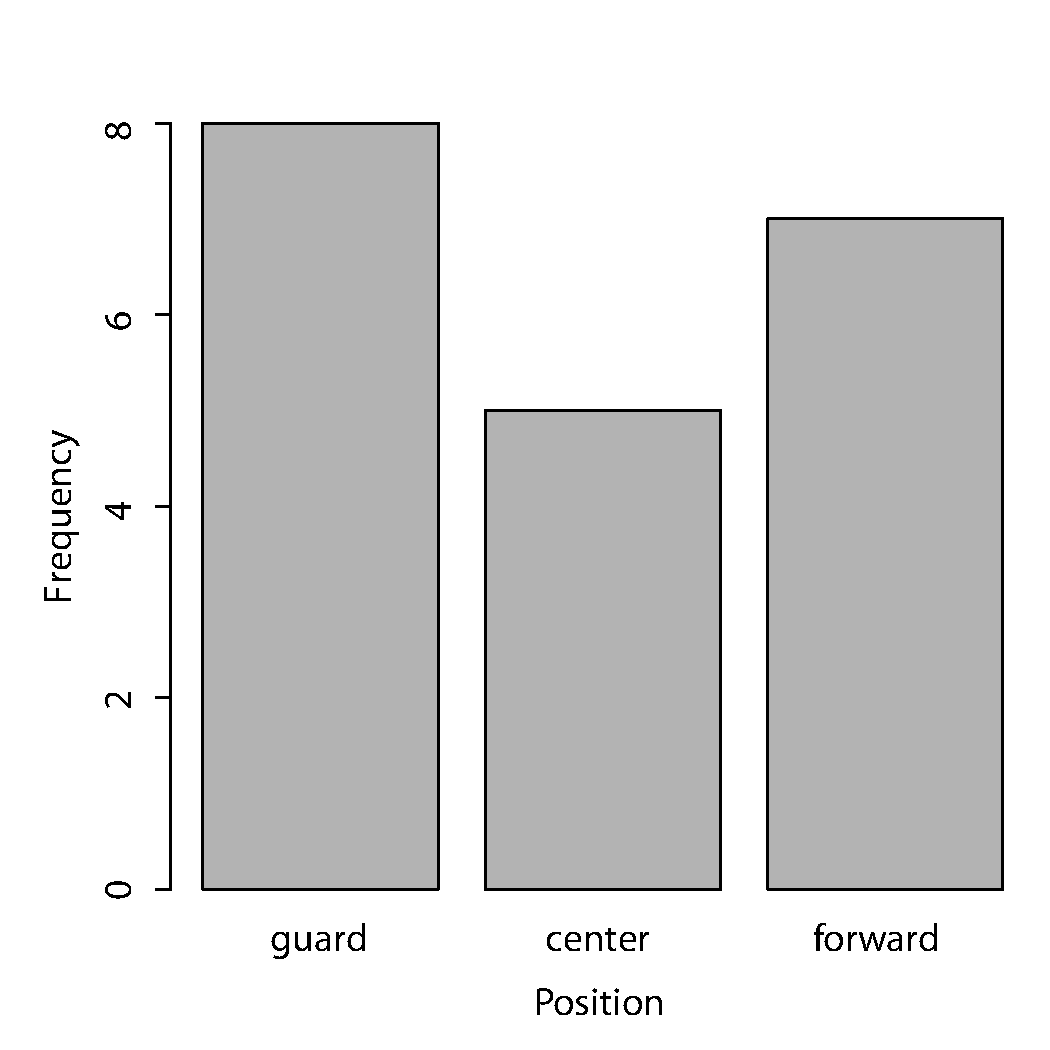
\includegraphics[width=0.32\textwidth]{./images/DataEx-CatVisEx1.pdf}} 
\subfigure[Proportion]{\label{fig:barPlotExProp}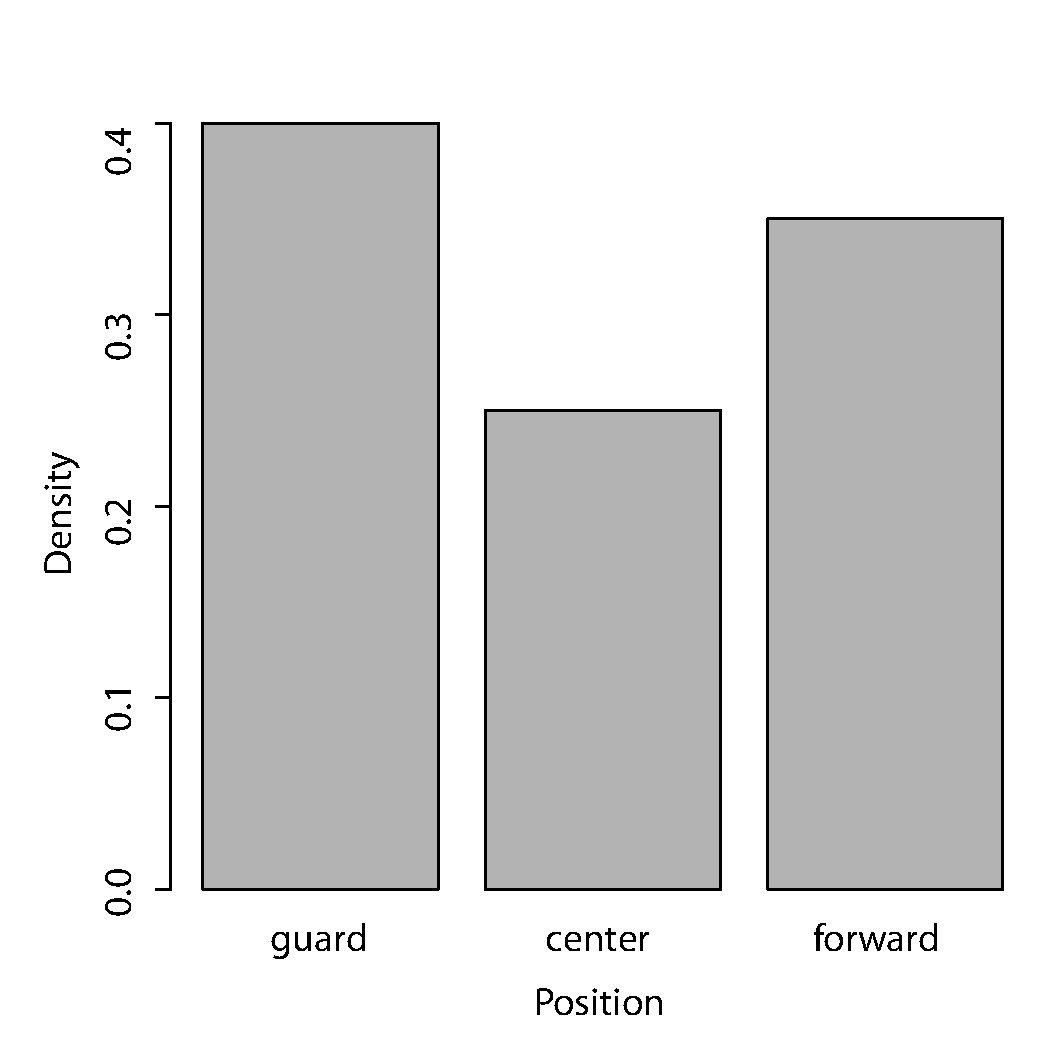
\includegraphics[width=0.32\textwidth]{./images/DataEx-CatVisEx2.pdf}} 
\subfigure[Ordered]{\label{fig:barPlotExOrdered}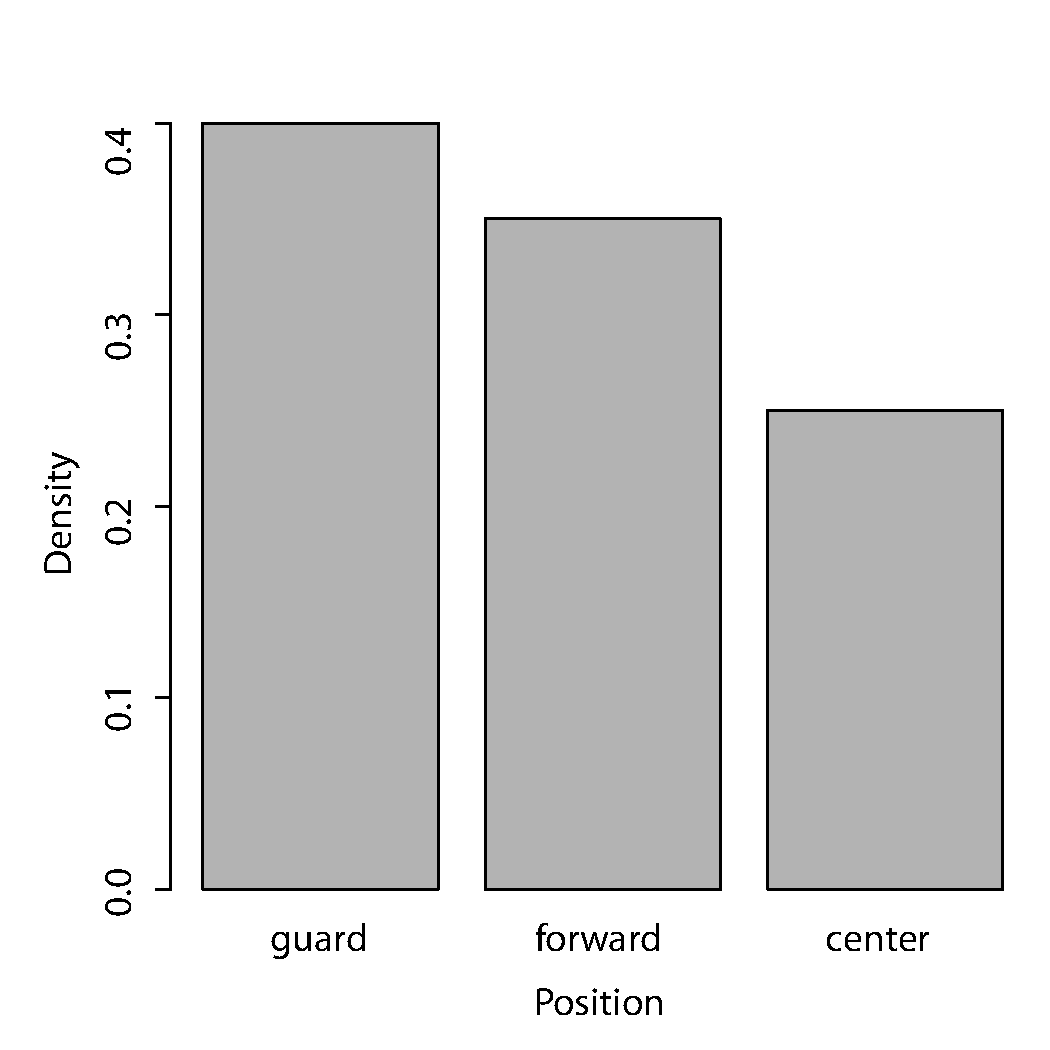
\includegraphics[width=0.32\textwidth]{./images/DataEx-CatVisEx3.pdf}} 
\end{center}
\label{fig:barPlotEx}
\end{figure}
\end{frame} 

\subsection{Histograms}

 \begin{frame} 
  \centering
 Bar plots don't work for continuous features
\begin{figure}[!htb]
\begin{centering}
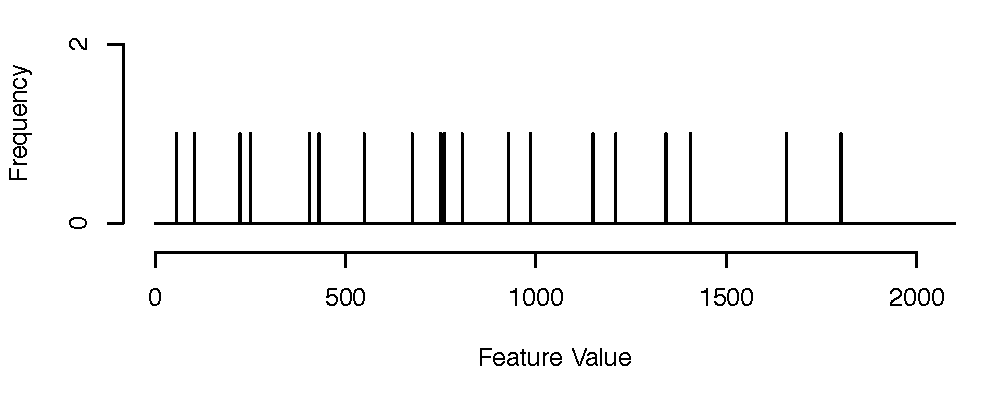
\includegraphics[width=0.65\textwidth]{./images/pdf_intro_3_small.pdf}
\label{fig:freq_hist_continuous}
\end{centering}
\end{figure}
\end{frame} 


 \begin{frame} [plain]
   \centering
 By dividing the range of a variable into intervals, or bins, we can generate \keyword{histograms}
 \begin{table}[!htb]
\label{table:densityCalculations}
\centering
\begin{scriptsize}
\subtable[200 unit intervals]{\label{table:densityCalculation10_200Intervals}\begin{tabular}{  l c r r }
\hline
\textbf{Interval} & \textbf{Count} & \textbf{Density} & \textbf{Prob}\\
\hline
$[0,200)$ & 2 & 0.0005 & 0.1\\
$[200,400)$ & 2 & 0.0005 & 0.1\\
$[400,600)$ & 3 & 0.00075 & 0.15\\
$[600,800)$ & 4 & 0.001 & 0.2\\
$[800,1000)$ & 3 & 0.00075 & 0.15\\
$[1000,1200)$ & 1 & 0.00025 & 0.05\\
$[1200,1400)$ & 2 & 0.0005 & 0.1\\
$[1400,1600)$ & 1 & 0.00025 & 0.05\\
$[1600,1800)$ & 1 & 0.00025 & 0.05\\
$[1800,2000)$  & 1 & 0.00025 & 0.02\\
\hline
\end{tabular}}
\subtable[500 unit intervals]{\label{table:densityCalculation4_500Intervals}\begin{tabular}{  l c l l  }
\hline
\textbf{Interval} & \textbf{Count} & \textbf{Density} & \textbf{Prob}\\
\hline
$[0,500)$ & 6 & 0.0006 & 0.3 \\
$[500,1000)$ & 8 &   0.0008 & 0.4 \\
$[1000,1500)$ & 4 & 0.0004 & 0.2 \\
$[1500,2000)$ & 2 &  0.0002 & 0.1 \\
\hline
\end{tabular}}
\end{scriptsize}
\end{table}
\end{frame} 

 \begin{frame} [plain]
\begin{figure}[!htb]
\centering
\subfigure{\label{fig:int_freq_hist_continuous_10_200}\includegraphics[width=0.45\textwidth]{./images/pdf_intro_5.pdf}}
\subfigure{\label{fig:int_freq_hist_continuous_4_500}\includegraphics[width=0.45\textwidth]{./images/pdf_intro_6.pdf}}
\subfigure{\label{fig:density_10_200}\includegraphics[width=0.45\textwidth]{./images/pdf_intro_7b.pdf}} 
\subfigure{\label{fig:density_4_500}\includegraphics[width=0.45\textwidth]{./images/pdf_intro_8b.pdf}}
\caption{Frequency and density histograms for the continuous Training Expenses feature from Table \ourRef{table:positionsAndExpenses}.}
\label{fig:prob_mass_discrete_v_continuous}
\end{figure}
\end{frame} 

\subsection{Box Plots}

 \begin{frame} 
 \keyword{Box plots} are another useful way of visualising continuous variables
 \begin{figure}
\centering
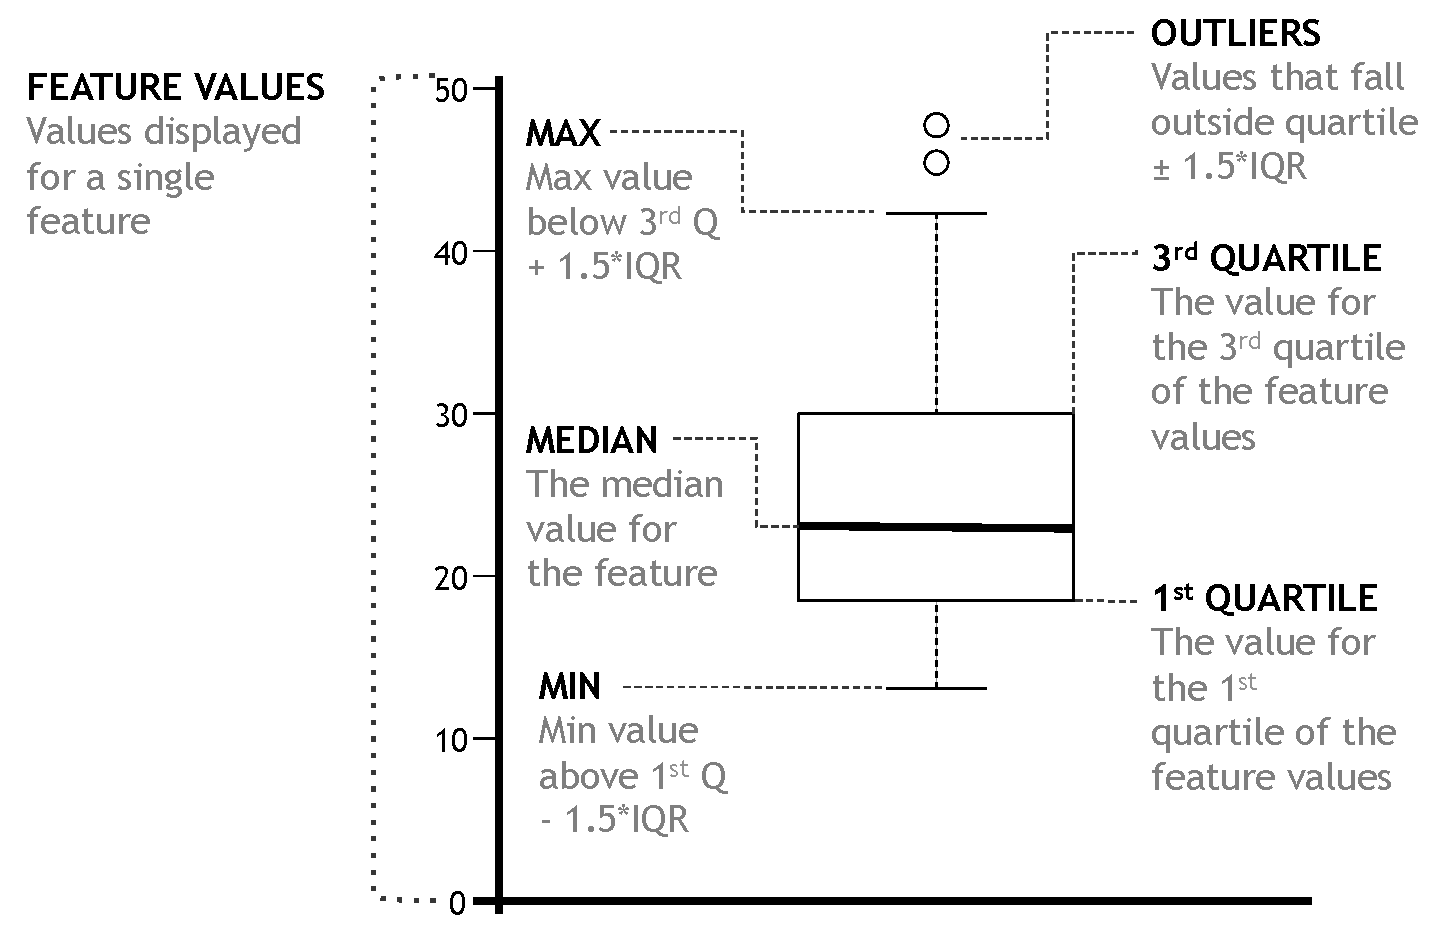
\includegraphics[width=0.6\textwidth]{./images/DataEx-BoxPlotStructure3.pdf}
\caption{The structure of a box plot.}
\label{fig:boxPlotStructure}
\end{figure}
\end{frame} 

 \begin{frame} 
 \begin{figure}
\centering
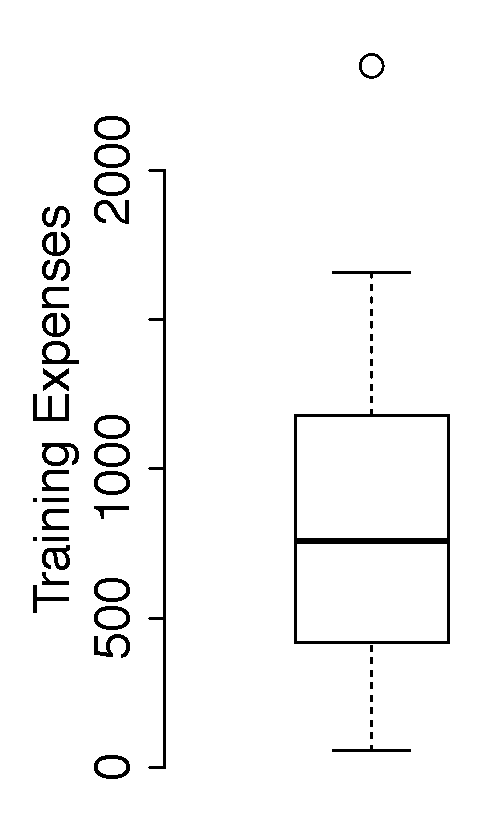
\includegraphics[width=0.3\textwidth]{./images/DataEx-BasketballSmallBoxPlot_TraingExpenses.pdf}
\caption{A box plot for the \featN{Training Expenses} feature from the basketball squad dataset in Table \ourRef{table:positionsAndExpenses}.}
\label{fig:boxPlotExample}
\end{figure}
\end{frame} 

\SectionSlide{Summary}

\begin{frame}
	\tableofcontents
\end{frame}

\end{document}
